

%% AAPT Physics Olympiad F=ma Questions
%%----------------------------------------


%% this section contains 39 problems


%% PhysicsOlympiad 2015
%%----------------------------------------
\element{aapt}{ %% Olympiad-A4
\begin{question}{Olympiad-2015-Q03}
    The force of friction on an airplane in level flight is given by $F_f = kv^2$,
        where $k$ is some constant, and $v$ is the speed of the airplane.
    When the power output from the engines is $P_0$,
        the plane is able to fly at a speed $v_0$.
    If the power output of the engines is increased by \SI{100}{\percent} to $2P_0$,
        the airplane will be able to fly at a new speed given by:
    \begin{multicols}{3}
    \begin{choices}
        \wrongchoice{$1.12 v_0$}
      \correctchoice{$1.26 v_0$}
        \wrongchoice{$1.41 v_0$}
        \wrongchoice{$2.82 v_0$}
        \wrongchoice{$8 v_0$}
    \end{choices}
    \end{multicols}
\end{question}
}



%% PhysicsOlympiad 2014
%%----------------------------------------
\element{aapt}{ %% Olympiad-A4
\begin{question}{Olympiad-2014-Q11}
    A point mass $m$ is connected to an ideal spring on a horizontal frictionless surface.
    The mass is pulled a short distance and then released.
    Which of the following is the most correct plot of the kinetic energy
        as a function of potential energy?
    \begin{multicols}{2}
    \begin{choices}
        \AMCboxDimensions{down=-1.00cm}
        \wrongchoice{
            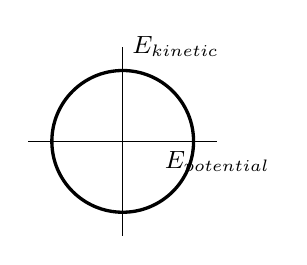
\begin{tikzpicture}[scale=0.60,font=\small]
                \draw (-2,0) -- (+2,0) node[anchor=north] {$E_{potential}$};
                \draw (0,-2) -- (0,+2) node[anchor=west] {$E_{kinetic}$};
                \draw[very thick] (0,0) circle (1.5cm);
            \end{tikzpicture}
        }
        \wrongchoice{
            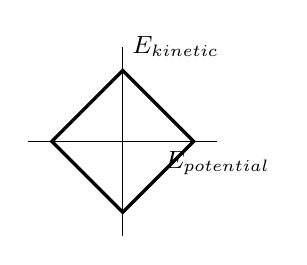
\begin{tikzpicture}[scale=0.60,font=\small]
                \draw (-2,0) -- (+2,0) node[anchor=north] {$E_{potential}$};
                \draw (0,-2) -- (0,+2) node[anchor=west] {$E_{kinetic}$};
                \draw[very thick] (-1.5,0) -- (0,1.5) -- (1.5,0) -- (0,-1.5) -- cycle;
            \end{tikzpicture}
        }
        \wrongchoice{
            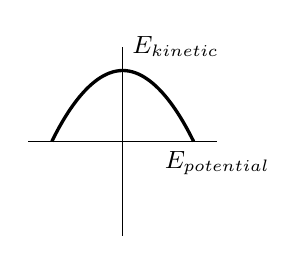
\begin{tikzpicture}[scale=0.60,font=\small]
                \draw (-2,0) -- (+2,0) node[anchor=north] {$E_{potential}$};
                \draw (0,-2) -- (0,+2) node[anchor=west] {$E_{kinetic}$};
                \draw[very thick] (-1.5,0) parabola bend (0,1.5) (1.5,0);
            \end{tikzpicture}
        }
        \wrongchoice{
            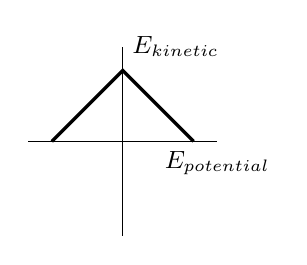
\begin{tikzpicture}[scale=0.60,font=\small]
                \draw (-2,0) -- (+2,0) node[anchor=north] {$E_{potential}$};
                \draw (0,-2) -- (0,+2) node[anchor=west] {$E_{kinetic}$};
                \draw[very thick] (-1.5,0) -- (0,1.5) -- (1.5,0);
            \end{tikzpicture}
        }
        %% ANS: E
        \correctchoice{
            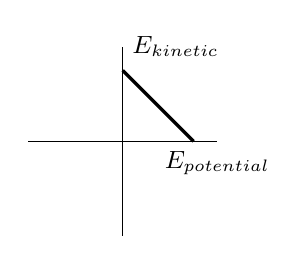
\begin{tikzpicture}[scale=0.60,font=\small]
                \draw (-2,0) -- (+2,0) node[anchor=north] {$E_{potential}$};
                \draw (0,-2) -- (0,+2) node[anchor=west] {$E_{kinetic}$};
                \draw[very thick] (0,1.5) -- (1.5,0);
            \end{tikzpicture}
        }
    \end{choices}
    \end{multicols}
\end{question}
}

\element{aapt}{ %% Olymmpiad-A4
\begin{question}{Olympiad-2014-Q25}
    A block with mass $m$ is released from rest at the top of a frictionless ramp.
    The block starts at a height $h_1$ above the base of the ramp,
        slides down the ramp, and then up a second ramp.
    The coefficient of kinetic friction between the block and the second ramp is $\mu_k$.
    If both ramps make an angle of $\theta$ with the horizontal,
        to what height $h_2$ above the base of the second ramp will the block rise?
    \begin{choices}
      \correctchoice{$h_2 = \dfrac{h_1\sin\theta}{\mu_k \cos\theta + \sin\theta}$}
        \wrongchoice{$h_2 = \dfrac{h_1\sin\theta}{\mu_k + \sin\theta}$}
        \wrongchoice{$h_2 = \dfrac{h_1\sin\theta}{\mu_k \cos^2\theta + \sin\theta}$}
        \wrongchoice{$h_2 = \dfrac{h_1\sin\theta}{\mu_k \cos^2\theta + \sin^2\theta}$}
        \wrongchoice{$h_2 = \dfrac{h_1\sin\theta}{\mu_k \sin\theta + \cos\theta}$}
    \end{choices}
\end{question}
}


%% PhysicsOlympiad 2013
%%----------------------------------------
\element{aapt}{ %% Olympiad-A4
\begin{question}{Olympiad-2013-Q23}
    %The following information applies to questions 23 and 24
    A man with mass $m$ jumps off of a high bridge with a bungee cord attached to his ankles.
    The man falls through a maximum distance $H$ at which point the bungee cord brings him to a momentary rest before he bounces back up.
    The bungee cord is perfectly elastic,
        obeying Hooke's force law with a spring constant $k$,
        and stretches from an original length of $L_0$ to a final length $L = L_0 + h$.
    The maximum tension in the Bungee cord is four times the weight of the man.
    %% Start question
    Determine the spring constant $k$.
    \begin{multicols}{2}
    \begin{choices}
        \wrongchoice{$k = \dfrac{mg}{h}$}
        \wrongchoice{$k = \dfrac{2mg}{h}$}
        \wrongchoice{$k = \dfrac{mg}{H}$}
        \wrongchoice{$k = \dfrac{2mg}{H}$}
      \correctchoice{$k = \dfrac{8mg}{H}$}
    \end{choices}
    \end{multicols}
\end{question}
}

\element{aapt}{ %% Olympiad-A4
\begin{question}{Olympiad-2013-Q24}
    %The following information applies to questions 23 and 24
    A man with mass $m$ jumps off of a high bridge with a bungee cord attached to his ankles.
    The man falls through a maximum distance $H$ at which point the bungee cord brings him to a momentary rest before he bounces back up.
    The bungee cord is perfectly elastic,
        obeying Hooke's force law with a spring constant $k$,
        and stretches from an original length of $L_0$ to a final length $L = L_0 + h$.
    The maximum tension in the Bungee cord is four times the weight of the man.
    %% Start question
    Find the maximum extension of the bungee cord $h$.
    \begin{multicols}{2}
    \begin{choices}
      \correctchoice{$h = \dfrac{1}{2}H$}
        \wrongchoice{$h = \dfrac{1}{4}H$}
        \wrongchoice{$h = \dfrac{1}{5}H$}
        \wrongchoice{$h = \dfrac{2}{5}H$}
        \wrongchoice{$h = \dfrac{1}{8}H$}
    \end{choices}
    \end{multicols}
\end{question}
}


%% PhysicsOlympiad 2012
%%----------------------------------------
\element{aapt}{ %% Olympiad-A4
\begin{question}{Olympiad-2012-Q08}
    A block of mass $m=\SI{3.0}{\kilo\gram}$ is moving on a horizontal surface
        towards a massless spring with spring constant $k=\SI{80.0}{\newton\per\meter}$.
    The coefficient of kinetic friction between the block and the
        surface is $\mu_k=\num{0.50}$.
    The block has a speed of \SI{2.0}{\meter\per\second} when it first
        comes in contact with the spring.
    How far will the spring be compressed?
    \begin{multicols}{3}
    \begin{choices}
        \wrongchoice{\SI{0.19}{\meter}}
      \correctchoice{\SI{0.24}{\meter}}
        \wrongchoice{\SI{0.39}{\meter}}
        \wrongchoice{\SI{0.40}{\meter}}
        \wrongchoice{\SI{0.61}{\meter}}
    \end{choices}
    \end{multicols}
\end{question}
}

\element{aapt}{ %% Olympiad-A4
\begin{question}{Olympiad-2012-Q13}
    Shown below is a graph of the $x$ component of force versus position
        for a \SI{4.0}{\kilo\gram} cart constrained to move in one dimension on the $x$ axis.
    \begin{center}
    \begin{tikzpicture}
        \begin{axis}[
            axis y line=middle,
            axis x line=bottom,
            axis line style={->},
            xlabel={$x$},
            x unit=\si{\meter},
            xtick={-4,-2,0,2,4,6,8},
            minor x tick num=1,
            ylabel={$F$},
            y unit=\si{\newton},
            ytick={-2,0,2,4,6},
            minor x tick num=1,
            grid=major,
            xmin=-2,ymax=8,
            ymin=-4,xmax=8,
            width=0.95\columnwidth,
            height=0.618\columnwidth,
        ]
        \addplot[line width=1pt,domain=-4:1]{5};
        \addplot[line width=1pt,domain=1:8]{6 - x};
        \end{axis}
    \end{tikzpicture}
    \end{center}
    At $x=0$ the cart has a velocity of \SI{-3.0}{\meter\per\second}
        (in the negative direction).
    Which of the following is closest to the maximum speed of the cart?
    \begin{multicols}{2}
    \begin{choices}
        \wrongchoice{\SI{1.6}{\meter\per\second}}
        \wrongchoice{\SI{2.5}{\meter\per\second}}
        \wrongchoice{\SI{3.0}{\meter\per\second}}
        \wrongchoice{\SI{4.0}{\meter\per\second}}
      \correctchoice{\SI{4.2}{\meter\per\second}}
    \end{choices}
    \end{multicols}
\end{question}
}

\element{aapt}{ %% Olympiad-A4
\begin{question}{Olympiad-2012-Q15}
    A car of mass $m$ has an engine that provides a constant power output $P$.
    Assuming no friction, what is the maximum constant speed $v_{max}$
        that this car can drive up a long incline that makes an angle θ with the horizontal?
    \begin{choices}
      \correctchoice{$v_{max}=\dfrac{P}{mg\sin\theta}$}
        \wrongchoice{$v_{max}=\dfrac{P^2\sin\theta}{mg}$}
        \wrongchoice{$v_{max}=\dfrac{1}{\sin\theta}\sqrt{\dfrac{2P}{mg}}$}
        \wrongchoice{There is no maximum constant speed.}
        \wrongchoice{The maximum constant speed depends on the length of the incline.}
    \end{choices}
\end{question}
}

\element{aapt}{ %% Olympiad-A4
\begin{question}{Olympiad-2012-Q19}
    A \SI{1 500}{\watt} motor is used to pump water a vertical height of
        \SI{2.0}{\meter} out of a flooded basement through a cylindrical pipe.
    The water is ejected though the end of the pipe at a speed of \SI{2.5}{\meter\per\second}.
    Ignoring friction and assuming that all of the energy of the motor goes to the water,
        which of the following is the closest to the radius of the pipe?
    The density of water is $\rho=\SI{1000}{\kilo\gram\per\meter\cubed}$.
    \begin{multicols}{3}
    \begin{choices}
        \wrongchoice{\SI{1/3}{\centi\meter}}
        \wrongchoice{\SI{1}{\centi\meter}}
        \wrongchoice{\SI{3}{\centi\meter}}
      \correctchoice{\SI{10}{\centi\meter}}
        \wrongchoice{\SI{30}{\centi\meter}}
    \end{choices}
    \end{multicols}
\end{question}
}


%% PhysicsOlympiad 2011
%%----------------------------------------
\element{aapt}{ %% Olympiad-A4
\begin{question}{Olympiad-2011-Q09}
    A spring has an equilibrium length of \SI{2.0}{\meter}
        and a spring constant of \SI{10}{\newton\per\meter}.
    Alice is pulling on one end of the spring with a force of \SI{3.0}{\newton}.
    Bob is pulling on the opposite end of the spring with a force of \SI{3.0}{\newton},
        in the opposite direction.
    What is the resulting length of the spring?
    \begin{multicols}{3}
    \begin{choices}
        \wrongchoice{\SI{1.7}{\meter}}
        \wrongchoice{\SI{2.0}{\meter}}
      \correctchoice{\SI{2.3}{\meter}}
        \wrongchoice{\SI{2.6}{\meter}}
        \wrongchoice{\SI{8.0}{\meter}}
    \end{choices}
    \end{multicols}
\end{question}
}

\element{aapt}{ %% Olympiad-A4
\begin{question}{Olympiad-2011-Q15}
    A vertical mass-spring oscillator is displaced \SI{2.0}{\centi\meter} from equilibrium.
    The \SI{100}{\gram} mass passes through the equilibrium point
        with a speed of \SI{0.75}{\meter\per\second}.
    What is the spring constant of the spring?
    \begin{multicols}{2}
    \begin{choices}
        \wrongchoice{\SI{90}{\newton\per\meter}}
        \wrongchoice{\SI{100}{\newton\per\meter}}
        \wrongchoice{\SI{110}{\newton\per\meter}}
      \correctchoice{\SI{140}{\newton\per\meter}}
        \wrongchoice{\SI{160}{\newton\per\meter}}
    \end{choices}
    \end{multicols}
\end{question}
}

\element{aapt}{ %% Olympiad-A4
\begin{question}{Olympiad-2011-Q18}
    A block of mass $m=\SI{3.0}{\kilo\gram}$ slides down one ramp, and then up a second ramp.
    The coefficient of kinetic friction between the block and each ramp is $\mu_k=\num{0.40}$.
    The block begins at a height $h_1=\SI{1.0}{\meter}$ above the horizontal.
    Both ramps are at a \ang{30} incline above the horizontal.
    To what height above the horizontal does the block rise on the second ramp?
    \begin{multicols}{3}
    \begin{choices}
      \correctchoice{\SI{0.18}{\meter}}
        \wrongchoice{\SI{0.52}{\meter}}
        \wrongchoice{\SI{0.59}{\meter}}
        \wrongchoice{\SI{0.69}{\meter}}
        \wrongchoice{\SI{0.71}{\meter}}
    \end{choices}
    \end{multicols}
\end{question}
}


%% PhysicsOlympiad 2010
%%----------------------------------------
\element{aapt}{ %% Olympiad-A4
\begin{question}{Olympiad-2010-Q12}
    A ball with mass $m$ projected horizontally off the end of a table
        with an initial kinetic energy $K$.
    At a time $t$ after it leaves the end of the table it has kinetic energy $3K$.
    What is $t$?
    Neglect air resistance
    \begin{multicols}{2}
    \begin{choices}
        \wrongchoice{$\dfrac{3}{g}\sqrt{\dfrac{K}{m}}$}
      \correctchoice{$\dfrac{2}{g}\sqrt{\dfrac{K}{m}}$}
        \wrongchoice{$\dfrac{1}{g}\sqrt{\dfrac{8K}{m}}$}
        \wrongchoice{$\dfrac{K}{g}\sqrt{\dfrac{6}{m}}$}
        \wrongchoice{$\dfrac{2K}{g}\sqrt{\dfrac{1}{m}}$}
    \end{choices}
    \end{multicols}
\end{question}
}

\newcommand{\olympiadTwentyTenQEighteen}{
\begin{tikzpicture}
    \begin{axis}[
        axis y line=left,
        axis x line=bottom,
        axis line style={->},
        xlabel={distance},
        x unit=\si{\meter},
        xtick={-15,-10,-5,0,5,10,15},
        ylabel={energy},
        y unit=\si{\joule},
        ytick={-10,-5,0},
        xmin=-16,xmax=16,
        ymin=-12,ymax=2,
        width=0.8\columnwidth,
        height=0.4\columnwidth,
        very thin,
    ]
    \addplot[line width=1pt,mark=\empty] plot coordinates {(-16,0) (-10,0) (0,-10) (10,0) (16,0)};
    \end{axis}
\end{tikzpicture}
}

\element{aapt}{ %% Olympiad-A4
\begin{question}{Olympiad-2010-Q18}
    The following is a graph of potential energy.
    \begin{center}
        \olympiadTwentyTenQEighteen
    \end{center}
    Which of the following represents the force corresponding to the given potential?
    \begin{choices}
        \AMCboxDimensions{down=-3.5em}
        \wrongchoice{
            \begin{tikzpicture}
                \begin{axis}[
                    axis y line=left,
                    axis x line=bottom,
                    axis line style={->},
                    xlabel={distance},
                    x unit=\si{\meter},
                    xtick={-15,-10,-5,0,5,10,15},
                    ylabel={force},
                    y unit=\si{\newton},
                    ytick={-2,-1,0,1,2},
                    xmin=-16,xmax=16,
                    ymin=-3,ymax=3,
                    width=0.8\columnwidth,
                    height=0.4\columnwidth,
                    very thin,
                ]
                \addplot[line width=1pt,mark=\empty] plot coordinates {(-16,0) (-10,0) (-10,-1) (0,-1) (0,1) (10,1) (10,0) ( 16,0)};
                \end{axis}
            \end{tikzpicture}
        }
        \wrongchoice{
            \begin{tikzpicture}
                \begin{axis}[
                    axis y line=left,
                    axis x line=bottom,
                    axis line style={->},
                    xlabel={distance},
                    x unit=\si{\meter},
                    xtick={-15,-10,-5,0,5,10,15},
                    ylabel={force},
                    y unit=\si{\newton},
                    ytick={-2,-1,0,1,2},
                    xmin=-16,xmax=16,
                    ymin=-3,ymax=3,
                    width=0.8\columnwidth,
                    height=0.4\columnwidth,
                    very thin,
                ]
                \addplot[line width=1pt,mark=\empty] plot coordinates {(-16,0) (-10,0) (-10,-2) (0,-2) (0,2) (10,2) (10,0) ( 16,0)};
                \end{axis}
            \end{tikzpicture}
        }
        \wrongchoice{
            \begin{tikzpicture}
                \begin{axis}[
                    axis y line=left,
                    axis x line=bottom,
                    axis line style={->},
                    xlabel={distance},
                    x unit=\si{\meter},
                    xtick={-15,-10,-5,0,5,10,15},
                    ylabel={force},
                    y unit=\si{\newton},
                    ytick={-2,-1,0,1,2},
                    xmin=-16,xmax=16,
                    ymin=-3,ymax=3,
                    width=0.8\columnwidth,
                    height=0.4\columnwidth,
                    very thin,
                ]
                \addplot[line width=1pt,mark=\empty] plot coordinates {(-16,0) (-10,0) (-10,-0.5) (0,-0.5) (0,0.5) (10,0.5) (10,0) ( 16,0)};
                \end{axis}
            \end{tikzpicture}
        }
        \wrongchoice{
            \begin{tikzpicture}
                \begin{axis}[
                    axis y line=left,
                    axis x line=bottom,
                    axis line style={->},
                    xlabel={distance},
                    x unit=\si{\meter},
                    xtick={-15,-10,-5,0,5,10,15},
                    ylabel={force},
                    y unit=\si{\newton},
                    ytick={-2,-1,0,1,2},
                    xmin=-16,xmax=16,
                    ymin=-3,ymax=3,
                    width=0.8\columnwidth,
                    height=0.4\columnwidth,
                    very thin,
                ]
                \addplot[line width=1pt,mark=\empty] plot coordinates {(-16,0) (-10,0) (-10,0.5) (0,0.5) (0,-0.5) (10,-0.5) (10,0) ( 16,0)};
                \end{axis}
            \end{tikzpicture}
        }
        %% ANS is E
        \correctchoice{
            \begin{tikzpicture}
                \begin{axis}[
                    axis y line=left,
                    axis x line=bottom,
                    axis line style={->},
                    xlabel={distance},
                    x unit=\si{\meter},
                    xtick={-15,-10,-5,0,5,10,15},
                    ylabel={force},
                    y unit=\si{\newton},
                    ytick={-2,-1,0,1,2},
                    xmin=-16,xmax=16,
                    ymin=-3,ymax=3,
                    width=0.8\columnwidth,
                    height=0.4\columnwidth,
                    very thin,
                ]
                \addplot[line width=1pt,mark=\empty] plot coordinates {(-16,0) (-10,0) (-10,1) (0,1) (0,-1) (10,-1) (10,0) ( 16,0)};
                \end{axis}
            \end{tikzpicture}
        }
    \end{choices}
\end{question}
}

\element{aapt}{ %% Olympiad-A4
\begin{questionmult}{Olympiad-2010-Q19}
    The following is a graph of potential energy.
    \begin{center}
        \olympiadTwentyTenQEighteen
    \end{center}
    Which of the graphs could be the motion of a particle in the given potential?
    \begin{choices}
        \AMCboxDimensions{down=-3.5em}
        \correctchoice{
            \begin{tikzpicture}
                \begin{axis}[
                    axis y line=left,
                    axis x line=bottom,
                    axis line style={->},
                    xlabel={time},
                    x unit=\si{\second},
                    xtick={0,2,4,6,8,10},
                    ylabel={position},
                    y unit=\si{\meter},
                    ytick={-10,0,10},
                    minor y tick num=1,
                    xmin=0,xmax=10.2,
                    ymin=-16,ymax=16,
                    width=0.8\columnwidth,
                    height=0.4\columnwidth,
                ]
                \addplot[line width=1pt,domain=0:10] {15};
                \end{axis}
            \end{tikzpicture}
        }
        \wrongchoice{
            \begin{tikzpicture}
                \begin{axis}[
                    axis y line=left,
                    axis x line=bottom,
                    axis line style={->},
                    xlabel={time},
                    x unit=\si{\second},
                    xtick={0,2,4,6,8,10},
                    ylabel={position},
                    y unit=\si{\meter},
                    ytick={-10,0,10},
                    minor y tick num=1,
                    xmin=0,xmax=10.2,
                    ymin=-16,ymax=16,
                    width=0.8\columnwidth,
                    height=0.4\columnwidth,
                ]
                \addplot[line width=1pt,domain=0:10] {-5};
                \end{axis}
            \end{tikzpicture}
        }
        \correctchoice{
            \begin{tikzpicture}
                \begin{axis}[
                    axis y line=left,
                    axis x line=bottom,
                    axis line style={->},
                    xlabel={time},
                    x unit=\si{\second},
                    xtick={0,2,4,6,8,10},
                    ylabel={position},
                    y unit=\si{\meter},
                    ytick={-10,0,10},
                    xmin=0,xmax=10.2,
                    ymin=-16,ymax=16,
                    width=0.8\columnwidth,
                    height=0.4\columnwidth,
                ]
                \addplot[line width=1pt,mark=\empty] plot coordinates {(0,10) (10,15) };
                \end{axis}
            \end{tikzpicture}
        }
    \end{choices}
\end{questionmult}
}

\element{aapt}{ %% Olympiad-A4
\begin{question}{Olympiad-2010-Q20}
    The following is a graph of potential energy.
    \begin{center}
        \olympiadTwentyTenQEighteen
    \end{center}
    Consider the following graph of position vs. time,
        which represents the motion of a certain particle in the given potential.
    \begin{center}
    \begin{tikzpicture}
        \begin{axis}[
            axis y line=left,
            axis x line=bottom,
            axis line style={->},
            xlabel={time},
            x unit=\si{\second},
            xtick={0,2,4,6,8,10},
            ylabel={position},
            y unit=\si{\meter},
            ytick={-5,0,5},
            xmin=0,xmax=10.2,
            ymin=-7,ymax=7,
            width=0.8\columnwidth,
            height=0.4\columnwidth,
        ]
        \addplot[line width=1pt,domain=0:10] {5*sin(0.785*deg(x)) };
        \end{axis}
    \end{tikzpicture}
    \end{center}
    What is the total energy of the particle?
    \begin{multicols}{3}
    \begin{choices}
      \correctchoice{\SI{-5}{\joule}}
        \wrongchoice{\SI{0}{\joule}}
        \wrongchoice{\SI{5}{\joule}}
        \wrongchoice{\SI{10}{\joule}}
        \wrongchoice{\SI{15}{\joule}}
    \end{choices}
    \end{multicols}
\end{question}
}


%% PhysicsOlympiad 2009
%%----------------------------------------
\element{aapt}{ %% Olympiad-A4
\begin{question}{Olympiad-2009-Q11}
    A \SI{2.25}{\kilo\gram} mass undergoes an acceleration as shown below.
    How much work is done on the mass?
    \begin{center}
    \begin{tikzpicture}
        \begin{axis}[
            axis y line=left,
            axis x line=middle,
            axis line style={->},
            xlabel={position},
            x unit=\si{\meter},
            xtick={0,2,4,6,8,10,12},
            minor x tick num=1,
            ylabel={acceleration},
            y unit=\si{\meter\per\second\squared},
            ytick={-2,0,2,4},
            minor x tick num=1,
            grid=major,
            xmin=0,xmax=12.5,
            ymin=-2.5,ymax=4.5,
            width=0.9\columnwidth,
            height=0.55\columnwidth,
        ]
        \addplot[line width=1pt,mark=\empty] plot coordinates { (0,0) (2,4) (4,4) (10,-2) (12,0) };
        \end{axis}
    \end{tikzpicture}
    \end{center}
    \begin{multicols}{3}
    \begin{choices}
      \correctchoice{\SI{36}{\joule}}
        \wrongchoice{\SI{22}{\joule}}
        \wrongchoice{\SI{5}{\joule}}
        \wrongchoice{\SI{-17}{\joule}}
        \wrongchoice{\SI{-36}{\joule}}
    \end{choices}
    \end{multicols}
\end{question}
}

\element{aapt}{ %% Olympiad-A4
\begin{question}{Olympiad-2009-Q12}
    Batman, who has a mass of $M=\SI{100}{\kilo\gram}$,
        climbs to the roof of a \SI{30}{\meter} building
        and then lowers one end of a massless rope to his sidekick Robin.
    Batman then pulls Robin, who has a mass of $m=\SI{75}{\kilo\gram}$,
        up the roof of the building.
    Approximately how much total work has Batman done after Robin is on the roof?
    \begin{multicols}{2}
    \begin{choices}
        \wrongchoice{\SI{60}{\joule}}
        \wrongchoice{\SI{7e3}{\joule}}
      \correctchoice{\SI{5e4}{\joule}}
        \wrongchoice{\SI{600}{\joule}}
        \wrongchoice{\SI{3e4}{\joule}}
    \end{choices}
    \end{multicols}
\end{question}
}


%% PhysicsOlympiad 2008
%%----------------------------------------
\element{aapt}{ %% Olympiad-A4
\begin{question}{Olympiad-2008-Q16}
    A massless spring with spring constant $k$ is vertically mounted so that
        bottom end is firmly attached to the ground, and the top end free.
    A ball with mass $m$ falls vertically down on the top end of the spring,
        becoming attached, so that the ball oscillates vertically on the spring.
    What equation describes the acceleration $a$ of the ball when it is at a height $y$
        above the original position of the top end of the spring?
    Let down be negative, and neglect air resistance;
        $g$ is the magnitude of the acceleration of free fall.
    \begin{multicols}{2}
    \begin{choices}
        \wrongchoice{$a = \dfrac{mv^2}{y} + g$}
        \wrongchoice{$a = \dfrac{mv^2}{k} - g$}
        \wrongchoice{$a = \dfrac{ky}{m} + g$}
        \wrongchoice{$a = -\dfrac{ky}{m} + g$}
      \correctchoice{$a = -\dfrac{ky}{m} - g$}
    \end{choices}
    \end{multicols}
\end{question}
}

\element{aapt}{ %% Olympiad-A4
\begin{question}{Olympiad-2008-Q17}
    A mass $m$ is resting at equilibrium suspended from a vertical spring
        of natural length $L$ and spring constant $k$ inside a box as shown:
    \begin{center}
    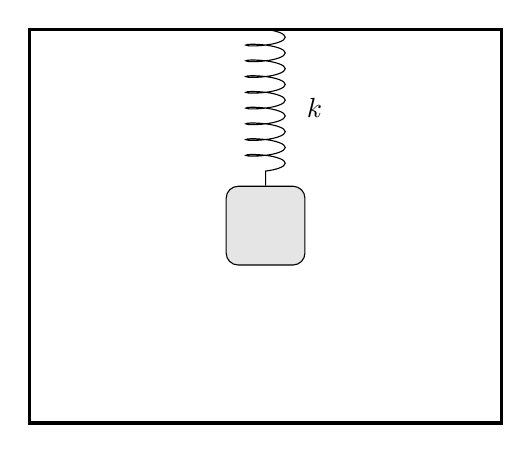
\begin{tikzpicture}
        %% Box
        \draw[very thick] (-3,0) rectangle (+3,-5);
        %% Blocks
        \node[draw,fill=white!90!black,rectangle,rounded corners=1ex,minimum size=1.00cm,anchor=south] (M) at (0,-3) {};
        %% Spring, Rope
        \draw[decoration={aspect=0.2,segment length=2.0mm,amplitude=2.5mm,coil},decorate] (0,0) -- (M.north) node[pos=0.5,anchor=west,xshift=4mm] {$k$};
    \end{tikzpicture}
    \end{center}
    The box begins accelerating upward with acceleration $a$.
    How much closer does the equilibrium position of the mass move to the bottom of the box?
    \begin{multicols}{3}
    \begin{choices}
        \wrongchoice{$\dfrac{aL}{g}$}
        \wrongchoice{$\dfrac{aL}{a}$}
        \wrongchoice{$\dfrac{m(g+a)}{k}$}
        \wrongchoice{$\dfrac{m(g-a)}{k}$}
      \correctchoice{$\dfrac{ma}{k}$}
    \end{choices}
    \end{multicols}
\end{question}
}


\element{aapt}{ %% Olympiad-A4
\begin{question}{Olympiad-2008-Q19}
    A car has an engine which delivers a constant power.
    It accelerates from rest at time $t=0$, and at $t=t_0$ its acceleration is $a_0$.
    What is its acceleration at $t = 2t_0$?
    Ignore energy loss due to friction.
    \begin{multicols}{3}
    \begin{choices}
        \wrongchoice{$\dfrac{1}{2}a_0$}
      \correctchoice{$\dfrac{1}{\sqrt{2}}a_0$}
        \wrongchoice{$a_0$}
        \wrongchoice{$\sqrt{2}a_0$}
        \wrongchoice{$2a_0$}
    \end{choices}
    \end{multicols}
\end{question}
}


%% PhysicsOlympiad 2007
%%----------------------------------------
\element{aapt}{ %% Olympiad-A4
\begin{question}{Olympiad-2007-Q07}
    The chemical potential energy stored in a battery is converted
        into kinetic energy in a toy car that increases its speed first
        from \SI{0}{\mile\per\hour} to \SI{2}{\mile\per\hour} and then from
        \SI{2}{\mile\per\hour} up to \SI{4}{\mile\per\hour}.
    Ignore the energy transferred to thermal energy due to friction and air resistance.
    Compared to the energy required to go from \SIrange{0}{2}{\mile\per\hour},
        the energy required to go from \SIrange{2}{4}{\mile\per\hour} is:
    \begin{choices}
        \wrongchoice{half the amount.}
        \wrongchoice{the same amount.}
        \wrongchoice{twice the amount.}
      \correctchoice{three times the amount.}
        \wrongchoice{four times the amount.}
    \end{choices}
\end{question}
}

\element{aapt}{ %% Olympiad-A4
\begin{question}{Olympiad-2007-Q18}
    A small chunk of ice falls from rest down a frictionless parabolic ice sheet shown in the figure.
    At the point labeled $A$ in the diagram,
        the ice sheet becomes a steady,
        rough incline of angle \ang{30} with respect to the horizontal and friction coefficient $\mu_k$.
    \begin{center}
    \begin{tikzpicture}[font=\small,scale=0.9]
        %% Surface
        \draw (0,0) -- (-4,0);
        \draw (0,0) -- (150:8) node[rotate=-30,pos=0.5,anchor=north] {rough incline};
        \draw (150:8) to[out=150,in=280] (-8,5.33);
        \node[draw,fill=white!90!black,rectangle,minimum size=1em,rotate=-80,anchor=south] (B) at (-8,5.33) {};
        \node[xshift=1ex,anchor=west] at (B.north) {ice chunk};
        %% Angle
        \draw (0,0) -- (180:1) arc(180:150:1) node[pos=0.5,anchor=east] {\ang{30}};
        %% Labels
        \draw[fill] (150:8) circle (1.5pt) node[anchor=south west] {$A$};
        \draw (0,0) -- (150:4);
        %% Length labels
        \draw[<->] (-9,0) -- (-9,5.33) node[pos=0.5,anchor=center,fill=white] {$h$};
        \draw[dashed,<->] (0,0) ++ (60:0.75) -- ++(150:8) node[pos=0.5,anchor=center,fill=white] {$\dfrac{3h}{2}$};
    \end{tikzpicture}
    \end{center}
    This incline is of length $\frac{3}{2}h$ and ends at a cliff.
    The chunk of ice comes to rest precisely at the end of the incline.
    What is the coefficient of friction $\mu_k$?
    \begin{multicols}{3}
    \begin{choices}
        \wrongchoice{\num{0.866}}
      \correctchoice{\num{0.770}}
        \wrongchoice{\num{0.667}}
        \wrongchoice{\num{0.385}}
        \wrongchoice{\num{0.333}}
    \end{choices}
    \end{multicols}
\end{question}
}

\element{aapt}{ %% Olympiad-A4
\begin{question}{Olympiad-2007-Q19}
    A non-Hookian spring has force $F=-kx^2$ where $k$ is the
        spring constant and $x$ is the displacement from its unstretched position.
    \begin{center}
    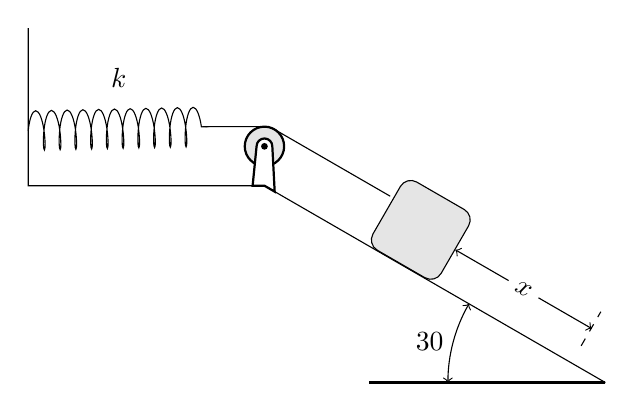
\begin{tikzpicture}
        %% NOTE: jphafner
        %% Surface
        \draw (-3,2) -- (-3,0) -- (0,0) -- (330:5);
        \draw[thick] (330:5) -- ++ (180:3);
        \draw[<->] (330:5) ++ (180:2) arc (180:150:2) node[pos=0.5,anchor=east] {\ang{30}};
        %% Blocks
        \node[draw,fill=white!90!black,rectangle,rounded corners=1ex,minimum size=1.00cm,rotate=-30,anchor=south] (M) at (330:2) {};
        %% Spring, Rope
        \draw[decoration={aspect=0.2,segment length=2.0mm,amplitude=2.5mm,coil},decorate] (-3,0.70) -- (-0.70,0.75) node[pos=0.5,anchor=south,yshift=4mm] {$k$};
        \draw (-0.75,0.75) -- (0,0.75) arc (90:60:0.25) -- ++(330:1.7);
        %% Pulley
        \draw[thick,fill=white!90!black] (0,0.5) circle (0.25);
        \draw[thick,fill=white] (-0.15,0) -- (-0.1,0.50) arc (180:0:0.1) -- (330:0.15) -- (0,0) -- cycle;
        \draw[fill] (0,0.5) circle (1pt);
        %% Displacement
        \draw[<->] (M.east) -- ++(330:2) node[pos=0.5,rotate=-30,anchor=center,fill=white] {$x$};
        \draw[dashed] (330:4.5) ++ (60:0.25) -- ++(60:0.5);
    \end{tikzpicture}
    \end{center}
    For the system shown of a mass $m$ connected to an
        unstretched spring initially at rest,
        how far does the spring extend before the system momentarily comes to rest?
    Assume that all surfaces are frictionless and that the pulley is frictionless as well.
    \begin{multicols}{2}
    \begin{choices}
      \correctchoice{$\left(\dfrac{3mg}{2k}\right)^{\dfrac{1}{2}}$}
        \wrongchoice{$\left(\dfrac{mg}{k}\right)^{\dfrac{1}{2}}$}
        \wrongchoice{$\left(\dfrac{2mg}{k}\right)^{\dfrac{1}{2}}$}
        \wrongchoice{$\left(\dfrac{\sqrt{3}mg}{k}\right)^{\dfrac{1}{3}}$}
        \wrongchoice{$\left(\dfrac{3\sqrt{3}mg}{2k}\right)^{\dfrac{1}{3}}$}
    \end{choices}
    \end{multicols}
\end{question}
}

\element{aapt}{ %% Olympiad-A4
\begin{question}{Olympiad-2007-Q20}
    A point-like mass moves horizontally between two walls on a
        frictionless surface with initial kinetic energy $E$.
    With every collision with the walls,
        the mass loses $\frac{1}{2}$ its kinetic energy to thermal energy.
    How many collisions with the walls are necessary before the
        speed of the mass is reduced by a factor of $8$?
    \begin{multicols}{3}
    \begin{choices}
        \wrongchoice{\num{3}}
        \wrongchoice{\num{4}}
      \correctchoice{\num{6}}
        \wrongchoice{\num{8}}
        \wrongchoice{\num{16}}
    \end{choices}
    \end{multicols}
\end{question}
}

\element{aapt}{ %% Olympiad-A4
\begin{question}{Olympiad-2007-Q22}
    Two rockets are in space in a negligible gravitational field.
    All observations are made by an observer in a reference frame
        in which both rockets are initially at rest.
    The masses of the rockets are $m$ and $9m$.
    A constant force $F$ acts on the rocket of mass $m$ for a distance $d$.
    As a result, the rocket acquires a momentum $p$.
    If the same constant force $F$ acts on the rocket of
        mass $9m$ for the same distance $d$,
        how much momentum does the rocket of mass $9m$ acquire?
    \begin{multicols}{3}
    \begin{choices}
        \wrongchoice{$\dfrac{p}{9}$}
        \wrongchoice{$\dfrac{p}{3}$}
        \wrongchoice{$p$}
      \correctchoice{$3 p$}
        \wrongchoice{$9 p$}
    \end{choices}
    \end{multicols}
\end{question}
}


%% PhysicsOlympiad 2004
%%----------------------------------------
\element{aapt}{ %% Olympiad-A4
\begin{question}{Olympiad-2004-Q06}
    It takes \SI{250}{\newton} to pull a longbow back \SI{0.6}{\meter}.
    If all the energy required to pull the bow back is delivered to the arrow,
        what would be the kinetic energy of the arrow when it is fired?
    Assume the bow behaves according to Hooke's law.
    \begin{multicols}{3}
    \begin{choices}
      \correctchoice{\SI{75}{\joule}}
        \wrongchoice{\SI{90}{\joule}}
        \wrongchoice{\SI{150}{\joule}}
        \wrongchoice{\SI{420}{\joule}}
        \wrongchoice{\SI{22 000}{\joule}}
    \end{choices}
    \end{multicols}
\end{question}
}


%% PhysicsOlympiad 2003
%%----------------------------------------
\element{aapt}{ %% Olympiad-A4
\begin{question}{Olympiad-2003-Q10}
    A roller coaster car moves along a track as shown.
    \begin{center}
    \begin{tikzpicture}
        %% Ground
        \node[anchor=north,fill,pattern=north east lines,minimum width=8cm, minimum height=0.05cm] at (3,0) {};
        \draw (-1,0) -- (7,0);
        %% Path
        \draw[thick] (-1,4.5) to[out=45,in=180] (0,5) to[out=0,in=180] (3,1) to[out=0,in=180] (6,3) to [out=0,in=145] (7,2.5);
        %% Mass
        \draw[thick] node[draw,rotate=30,fill=white!90!black,minimum size=0.5cm,anchor=south] (M) at (-0.6,4.8) {};
        \draw (M.south east) circle (0.1cm);
        \draw (M.south west) circle (0.1cm);
        %% Labels
        \node[anchor=south] at (-0,5) {$A$};
        \node[anchor=south] at (6,3) {$B$};
        \draw[<->] (0,0) -- (0,5) node[pos=0.5,fill=white,anchor=center] {\SI{50}{\meter}};
        \draw[<->] (3,0) -- (3,1) node[pos=0.5,fill=white,anchor=center] {\SI{10}{\meter}};
        \draw[<->] (6,0) -- (6,3) node[pos=0.5,fill=white,anchor=center] {\SI{30}{\meter}};
    \end{tikzpicture}
    \end{center}
    At point $A$,
        the roller coaster car is moving with a speed of \SI{10}{\meter\per\second}.
    If friction is negligible,
        about how fast would the car be moving at point $B$?
    \begin{multicols}{3}
    \begin{choices}
        \wrongchoice{\SI{14}{\meter\per\second}}
        \wrongchoice{\SI{20}{\meter\per\second}}
      \correctchoice{\SI{22}{\meter\per\second}}
        \wrongchoice{\SI{26}{\meter\per\second}}
        \wrongchoice{\SI{31}{\meter\per\second}}
    \end{choices}
    \end{multicols}
\end{question}
}

\element{aapt}{ %% Olympiad-A4
\begin{question}{Olympiad-2003-Q11}
    A laboratory cart with a mass of $m$ and velocity $v$ runs headlong into a stationary spring bumper and compresses the spring.
    If the spring has a spring constant $k$,
        what is the maximum compression of the spring?
    \begin{multicols}{3}
    \begin{choices}
      \correctchoice{$v \sqrt{\dfrac{m}{k}}$}
        \wrongchoice{$\sqrt{\dfrac{mv}{k}}$}
        \wrongchoice{$\dfrac{mv^2}{2k}$}
        \wrongchoice{$mv\sqrt{k}$}
        \wrongchoice{$\sqrt{\dfrac{mv}{2k}}$}
    \end{choices}
    \end{multicols}
\end{question}
}


%% PhysicsOlympiad 2000
%%----------------------------------------
\element{aapt}{ %% Olympiad-A4
\begin{question}{olympiad-2000-q10}
    An arrow is to be propelled by a simple bow.
    If the arrow were given a velocity $v$ by a certain displacement $d$,
        what would be the arrow's velocity with a displacement of $3d$?
    Assume the magnitude of the force the bow exerts on the arrow is proportional to the arrow displacement.
    \begin{multicols}{3}
    \begin{choices}
      \correctchoice{$3 v$}
        \wrongchoice{$6 v$}
        \wrongchoice{$9 v$}
        \wrongchoice{$12 v$}
        \wrongchoice{$27 v$}
    \end{choices}
    \end{multicols}
\end{question}
}

\element{aapt}{ %% Olympiad-A4
\begin{question}{olympiad-2000-q16}
    If projectile is fired vertically upward from the surface of Mercury
        ($g_{\text{Mercury}} = \SI{3.75}{\meter\per\second\squared}$),
    what would be the required initial velocity if the projectile is to rise to a maximum height of \SI{30}{\meter}?
    \begin{multicols}{3}
    \begin{choices}
        \wrongchoice{\SI{4.0}{\meter\per\second}}
        \wrongchoice{\SI{8.0}{\meter\per\second}}
        \wrongchoice{\SI{10.6}{\meter\per\second}}
      \correctchoice{\SI{15.0}{\meter\per\second}}
        \wrongchoice{\SI{11.2}{\meter\per\second}}
    \end{choices}
    \end{multicols}
\end{question}
}

\element{aapt}{ %% Olympiad-A4
\begin{question}{olympiad-2000-q18}
    %% Questions 17 and 18 refer to the situation shown in the accompanying diagram.
    Two \SI{5}{\kilo\gram} masses are attached to opposite ends of a long massless cord which passes tautly over a massless frictionless pulley.
    The upper mass is initially held at rest on a table \SI{50}{\centi\meter} from the pulley.
    The coefficient of kinetic friction between this mass and the table is \num{0.20}.
    \begin{center}
    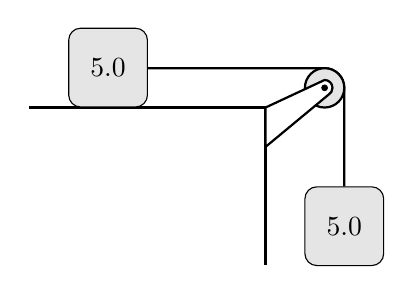
\begin{tikzpicture}
        %% Floor
        \draw[very thick] (-3,0) -- (0,0) -- (0,-2);
        %% Mass
        \node[draw,fill=white!90!black,rectangle,rounded corners=1ex,minimum size=1.0cm,anchor=south] (A) at (-2,0) {\SI{5.0}{\kilo\gram}};
        \node[draw,fill=white!90!black,rectangle,rounded corners=1ex,minimum size=1.0cm,anchor=north] (B) at (1,-1) {\SI{5.0}{\kilo\gram}};
        %% Rope and Pully
        \draw[thick] (A.south east) ++(90:0.5) -- (0.75,0.5) arc(90:0:0.25) -- (B.north);
        \draw[thick,fill=white!90!black] (0.75,0.25) circle (0.25);
        \draw[thick,fill=white] (0,0) -- (0.75,0.35) arc (90:-60:0.1) -- (0,-0.5) -- cycle;
        \draw[fill] (0.75,0.25) circle (1pt);
    \end{tikzpicture}
    \end{center}
    %% start question
    When the hanging mass has fallen a distance of \SI{30}{\centi\meter},
        how much work has been done by the frictional force?
    \begin{multicols}{3}
    \begin{choices}
        \wrongchoice{\SI{-147}{\joule}}
        \wrongchoice{\SI{-14.7}{\joule}}
        \wrongchoice{\SI{-9.8}{\joule}}
        \wrongchoice{\SI{-5.8}{\joule}}
      \correctchoice{\SI{-2.9}{\joule}}
    \end{choices}
    \end{multicols}
\end{question}
}

\element{aapt}{ %% Olympiad-A4
\begin{question}{olympiad-2000-q24}
    A small bird with a mass of \SI{0.5}{\kilo\gram} takes off from the ground and flies with an upward velocity of \SI{3}{\meter\per\second} for \SI{10}{\second}.
    Which of the following is closest to the minimum power that must be developed by the bird?
    \begin{multicols}{3}
    \begin{choices}
        \wrongchoice{\SI{60}{\watt}}
      \correctchoice{\SI{15}{\watt}}
        \wrongchoice{\SI{9}{\watt}}
        \wrongchoice{\SI{6}{\watt}}
        \wrongchoice{\SI{1.5}{\watt}}
    \end{choices}
    \end{multicols}
\end{question}
}


%% PhysicsOlympiad 1999
%%----------------------------------------
\element{aapt}{ %% Olympiad-A4
\begin{question}{olympiad-1999-q09}
    A driver in a \SI{1500}{\kilo\gram} sports car wishes to pass a slow moving truck on a two lane road.
    What is the average power required to accelerate the sports car from \SI{20}{\meter\per\second} to \SI{40}{\meter\per\second} in \SI{3}{\second}?
    \begin{multicols}{2}
    \begin{choices}
        \wrongchoice{\SI{10 000}{\watt}}
        \wrongchoice{\SI{20 000}{\watt}}
        \wrongchoice{\SI{100 000}{\watt}}
      \correctchoice{\SI{300 000}{\watt}}
        \wrongchoice{\SI{400 000}{\watt}}
    \end{choices}
    \end{multicols}
\end{question}
}

\element{aapt}{ %% Olympiad-A4
\begin{question}{olympiad-1999-q10}
    A \SI{40}{\kilo\gram} mass is attached to a horizontal spring with a constant of \SI{500}{\newton\per\meter}.
    If the mass rests on a frictionless horizontal surface,
        what is the total energy of this system when set into simple harmonic motion by an original displacement of \SI{0.2}{\meter}?
    \begin{multicols}{3}
    \begin{choices}
      \correctchoice{\SI{10}{\joule}}
        \wrongchoice{\SI{20}{\joule}}
        \wrongchoice{\SI{50}{\joule}}
        \wrongchoice{\SI{4000}{\joule}}
        \wrongchoice{\SI{100 000}{\joule}}
    \end{choices}
    \end{multicols}
\end{question}
}


%% PhysicsOlympiad 1996
%%----------------------------------------
\element{aapt}{ %% Olympiad-A4
\begin{question}{olympiad-1996-q11}
    A roller coaster travels with speed $v_A$ at point $A$.
    Point $B$ is a height $H$ above point $A$.
    Assuming no frictional losses and no work done by a motor,
        what is the speed at point $B$?
    \begin{multicols}{2}
    \begin{choices}
      \correctchoice{$\sqrt{v_A^2 - 2gH}$}
        \wrongchoice{$v_A - \sqrt{2gH}$}
        \wrongchoice{$v_A - 2gH$}
        \wrongchoice{$v_A + \sqrt{2gH}$}
        \wrongchoice{$\sqrt{v_A^2 + 2gH}$}
    \end{choices}
    \end{multicols}
\end{question}
}


%% PhysicsOlympiad 1995
%%----------------------------------------
\element{aapt}{ %% Olympiad-A4
\begin{question}{olympiad-1995-q05}
    A mass attached to a horizontal massless spring is displaced \SI{16}{\centi\meter} to the right of its equilibrium position and released from rest.
    At its \SI{16}{\centi\meter} extension,
        the spring-mass system has \SI{1.28}{\joule} of potential energy.
    \begin{center}
    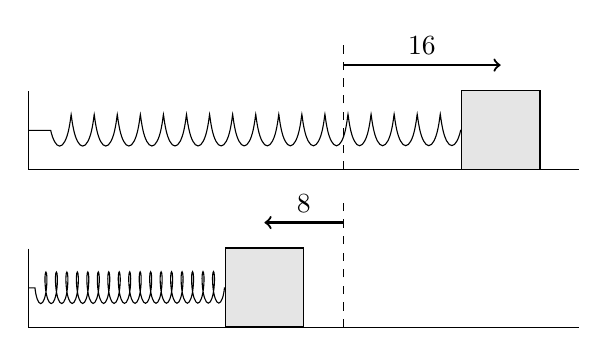
\begin{tikzpicture}
        \begin{scope}[yshift=1cm]
            %% Floor and Wall
            \draw (0,1) -- (0,0) -- (7,0);
            %% block
            \node[draw,fill=white!90!black,minimum size=1cm,anchor=south] (A) at (6,0) {};
            %% Spring
            \draw[decoration={aspect=0.2,segment length=2.93mm,amplitude=2mm,coil},decorate] (A.west) -- (0,0.5);
            %% midway
            \draw[dashed] (4,0) -- (4,1.66);
            \draw[thick,->] (4,1.33) -- (6,1.33) node[pos=0.5,anchor=south] {\SI{16}{\centi\meter}};
        \end{scope}
        \begin{scope}[yshift=-1cm]
            %% Floor and Wall
            \draw (0,1) -- (0,0) -- (7,0);
            %% block
            \node[draw,fill=white!90!black,minimum size=1cm,anchor=south] (A) at (3,0) {};
            %% Spring
            \draw[decoration={aspect=0.2,segment length=1.33mm,amplitude=2mm,coil},decorate] (A.west) -- (0,0.5);
            %% midway
            \draw[dashed] (4,0) -- (4,1.66);
            \draw[thick,->] (4,1.33) -- (3,1.33) node[pos=0.5,anchor=south] {\SI{8}{\centi\meter}};
        \end{scope}
    \end{tikzpicture}
    \end{center}
    Upon release, it slides across a rough surface and comes momentarily to rest \SI{8}{\centi\meter} to the left of its equilibrium position.
    How much mechanical energy was dissipated by friction?
    \begin{multicols}{3}
    \begin{choices}
        \wrongchoice{\SI{0.16}{\joule}}
        \wrongchoice{\SI{0.32}{\joule}}
        \wrongchoice{\SI{0.64}{\joule}}
      \correctchoice{\SI{0.96}{\joule}}
        \wrongchoice{\SI{1.12}{\joule}}
    \end{choices}
    \end{multicols}
\end{question}
}


%% PhysicsOlympiad 1994
%%----------------------------------------
\element{aapt}{ %% Olympiad-A4
\begin{question}{olympiad-1994-q07}
    A cube with mass $M$ starts at rest at point 1 at a height $4R$,
        where $R$ is the radius of the circular part of the track.
    The cube slides down the frictionless track and around the loop.
    \begin{center}
    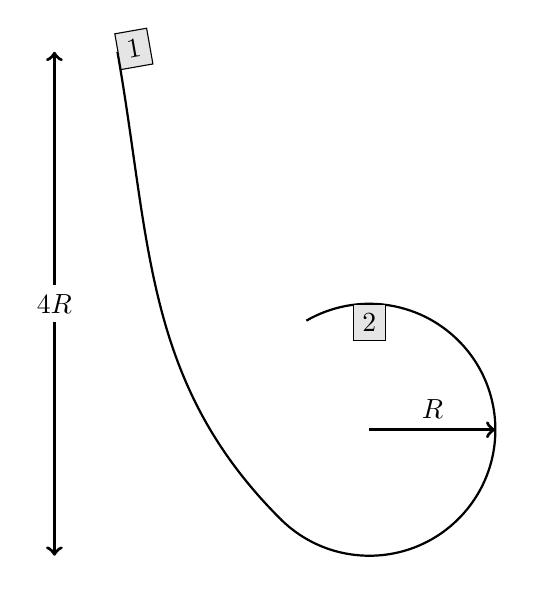
\begin{tikzpicture}[scale=0.8]
        %% Track
        \draw[thick] (-4,6) to[out=280,in=135] (225:2);
        \draw[thick] (225:2) arc(-135:120:2);
        \draw[very thick,->] (0,0) -- (2,0) node[pos=0.5,anchor=south] {$R$};
        %% block 1
        \node[draw,fill=white!90!black,minimum size=0.25,anchor=west,rotate=10] at (-4,6) {$1$};
        %% block 2
        \node[draw,fill=white!90!black,minimum size=0.25,anchor=north] at (90:2) {$2$};
        %% 6R
        \draw[very thick,<->] (-5,-2) -- (-5,6) node[pos=0.5,anchor=center,fill=white] {$4R$};
    \end{tikzpicture}
    \end{center}
    The force that the track exerts on the cube at point 2 is most nearly \rule[-0.1pt]{4em}{0.1pt} times the cube's weight $Mg$.
    \begin{multicols}{3}
    \begin{choices}
        \wrongchoice{1}
        \wrongchoice{2}
      \correctchoice{3}
        \wrongchoice{4}
        \wrongchoice{5}
    \end{choices}
    \end{multicols}
\end{question}
}

\element{aapt}{ %% Olympiad-A4
\begin{question}{olympiad-1994-q15}
    A block of mass $M$ is attached to a relaxed spring with force constant $k$,
        placed on a frictionless inclined plane as shown in the accompanying figure, and released.
    \begin{center}
    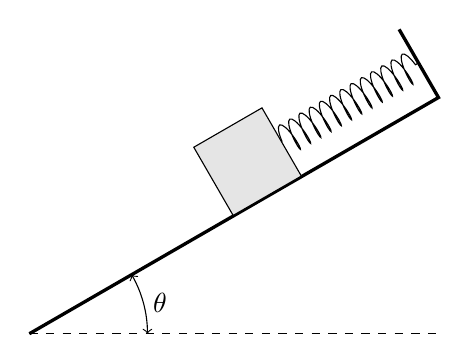
\begin{tikzpicture}
        %% incline
        \draw[very thick] (0,0) -- (30:6) --++(120:1);
        \draw[dashed] (0,0) -- (0:5.20);
        \draw[<->] (1.5,0) arc (0:30:1.5) node[pos=0.5,anchor=west] {$\theta$};
        %% block
        \node[draw,anchor=south east,minimum size=1cm,rotate=30,fill=white!90!black] (A) at (30:4) {};
        %% Spring
        \draw[decoration={aspect=0.2,segment length=1.5mm,amplitude=2mm,coil},decorate] (A.east) -- ++(30:2);
    \end{tikzpicture}
    \end{center}
    What is the maximum extension of the spring?
    \begin{multicols}{2}
    \begin{choices}
      \correctchoice{$x = \dfrac{2Mg\sin\theta}{k}$}
        \wrongchoice{$x = \dfrac{Mg\sin\theta}{k}$}
        \wrongchoice{$x = \dfrac{2Mg}{k}$}
        \wrongchoice{$x = \dfrac{Mg}{k}$}
        \wrongchoice{$x = \sqrt{2gM}$}
    \end{choices}
    \end{multicols}
\end{question}
}


\endinput


